%###############################################################################
% Plantilla de LaTeX no oficial de la Maestría en Economía - FCEA - UDELAR

% Adaptado al formato aprobado por la Comisión Académica de la Maestría en 
% Economía - FCEA - UDELAR

% Elaborado por: Juan Ignacio Urruty

% Inspirado en: 

% 1) Plantilla no oficilar de Udelar creada por LaTeXUy. En particular, Jorge 
% Pérez Zerpa (https://github.com/jorgepz), Mihdí Caballero 
% (https://github.com/mihdicaballero) y https://github.com/MBerguer   

% Pueden encontrar el repositorio original en: 
% https://github.com/LaTeXUy/UdelaRTeX 

% 2) Pautas de presentación y normalización de los Trabajos Académicos
% Elaboradas por las Bibliotecólogas Rita Grisolia y Fabiana Delfino

% Pueden encontrar el documento en el siguiente 
% (https://fcea.udelar.edu.uy/images/micrositios/biblioteca/PDF/Pautas_para_Trabajos_Finales_Acad%C3%A9micos.pdf) 

% 3) Plantilla de Word y LibreOffice creada por Sergio Palomeque

% Recursos adicionales:

% El estilo para las referencias bibliográficas en español fue realizada por 
% https://github.com/SantiPlanet

% Pueden encontrar el repositorio original en 
% https://github.com/SantiPlanet/apalike

%###############################################################################

%###############################################################################
% Preambulo - paquetes

% Aca se pone el tamaño de la fuente y el tipo de documento
\documentclass[11pt]{article}

% Esto sirve para manejar las citas bibliograficas
\usepackage[authoryear]{natbib}

% Esto configura las citas bibliográficas y las referencias en el estilo APA en 
% español. Le da un formato a lo que termina saliendo en la bibliografía y al 
% usar los comandos de \citet \citep \citeauthor \citeyear, etc.
\bibliographystyle{apalike-es.bst}

% Esto define a la fuente del texto con una fuente similar a la times new roman. 
% Además, pone que las expresiones matemáticas tengan esa misma fuente.
\usepackage{times}
\usepackage{mathptmx}

% Esto es para que el documento se encuentre seteado en español, por ejemplo: 
% hace aparecer la palabra "índice" la parte del índice en vez de la palabra 
% "contents"
\usepackage[spanish]{babel}

% Paquetes que ayudan con las tablas e imágenes
\usepackage{subfigure}
\usepackage{graphicx}
\usepackage{float}
\usepackage[labelfont=bf]{caption}
\usepackage[shortlabels]{enumitem}

% Esto pone en 5 el nivel de secciones que se incluyen en el índice
% 0 capitulo, 1 sección, 2 subsección, 3 subsubsección, 4 párrafo, 5 subpárrafo
\setcounter{tocdepth}{5}
\setcounter{secnumdepth}{5}

% Esto interactua con los comandos itemize, enumerate y description
\usepackage[shortlabels]{enumitem}

% Paquete que ayuda con las fórmulas matemáticas
\usepackage{amsmath}

% Esto es un paquete que le brinda unos nombres a los colores que se van a 
% utilizar en links por ejemplo
\usepackage[svgnames]{xcolor}

% Este paquete hace que los links tengan un color y lo establece como azul 
% oscuro (se puede cambiar) o quitar. Es recomendable dejar el paquete de 
% hyperref de todas formas \usepackage{hyperref}
\usepackage[colorlinks=true,allcolors=DarkBlue]{hyperref}

% Paquete para poder cambiar los márgenes
% Los márgenes establecidos por las pautas son de 2.5cm
% No modificar
\usepackage[a4paper]{geometry}
\geometry{top=2.5cm, bottom=2.5cm, left=2.5cm, right=2.5cm}

% Este paquete es para simplificar la vida con las citas con comillas hay que 
% poner \say{} y el texto
\usepackage{dirtytalk}

% Esto es para modificar el interlineado.
% En las primeras páginas se pondrá en 1.5. Para el cuerpo del archivo, en los
% capítulos, se pondrá espaciado doble.
\usepackage{setspace}
\onehalfspacing

% Se pueden agregar los paquetes adicionales que hagan falta para las
% necesidades particulares de cada tesis de maestría

%###############################################################################

%###############################################################################
% Comienzo del documento
\begin{document}

% Primera parte:
% Caratulas e integrantes del tribunal. En esta parte no debería quitarse 
% ninguna de las páginas, solamente modificar con los datos correspondientes: 
% titulo, nombres, tutora, cotutora, directora académica, mes de entrega, año 
% de entrega

% Esto es para que no se le ponga número a estas páginas y que las mismas no 
% aparezcan luego en el índice
\pagestyle{empty}
\pagenumbering{gobble}

\begin{center}

% Esta linea inserta los logos institucionales. Se recomienda
% no modificar
\noindent\makebox[\textwidth]{
\includegraphics[scale=0.5]{logos/Logos - FCEA - Depto - Udelar.jpg}}

% El comando vspace permite personalizar el espacio entre los diversos elementos
\vspace{1cm}

% Reemplazar por el título de la tesis luego del comando \Huge
\Huge Evaluación del impacto del título de la tesis: una mirada desde la plantilla de \LaTeX

\vspace{3cm}

% Reemplazar por Nombre y apellido luego del comando \Large
\Large Nombres y apellidos de la autora

\vspace{5cm}

% Dejar esto como está
\normalsize Programa de Maestría en Economía de la Facultad de Ciencias Económicas y de Administración

Universidad de la República

\vspace{2cm}

Montevideo - Uruguay

\vspace{0.5cm}

% Reemplazar por el mes y año de entrega de la tesis
(mes de entrega) de (año de entrega)
    
\end{center}

% Salto de página. Dejar este comando
\newpage

\begin{center}

% Esta linea inserta los logos institucionales. Se recomienda
% no modificar
\noindent\makebox[\textwidth]{
\includegraphics[scale=0.5]{logos/Logos - FCEA - Depto - Udelar.jpg}}

\vspace{0.5cm}

% Reemplazar por el título de la tesis luego del comando \Huge
\Huge Evaluación del impacto del título de la tesis: una mirada desde la plantilla de \LaTeX

\vspace{2cm}

% Reemplazar por Nombre y apellido luego del comando \Large
\Large Nombres y apellidos de la autora

\vspace{1cm}

\end{center}

% Dejar esto como está
\normalsize Tesis de Maestría presentada al Programa de Maestría en Economía de la Facultad de Ciencias Económicas y de Administración, Universidad de la República, como parte de los requisitos para la obtención del título de Magíster en Economía.

\vspace{1cm}

\begin{center}

% Cambiar en función de cada caso.
Directora de tesis: 

\vspace{1.5mm}

Ejemplo: Profesora Nombre Apellido

\vspace{6mm}

% Comentar en caso de no contar con codirectora
Codirectora de tesis: 

\vspace{1.5mm}

% Comentar en caso de no contar con codirectora
Ejemplo: Profesora Nombre Apellido

\vspace{6mm}

% Incluir esta información por más que
% la tutora y la directora académica coincidan
Directora académica: 

\vspace{1.5mm}

Ejemplo: Profesora Nombre Apellido

\vspace{1.5cm}

Montevideo - Uruguay

\vspace{0.5cm}

% Reemplazar por el mes y año de entrega de la tesis
(mes de entrega) de (año de entrega)

\end{center}

% Salto de página
\newpage

% Esta linea inserta los logos institucionales. Se recomienda
% no modificar
\noindent\makebox[\textwidth]{
\includegraphics[scale=0.5]{logos/Logos - FCEA - Depto - Udelar.jpg}}

% Se recomienda no modificar esta línea
\Large \underline{\textbf{Página de aprobación}}

\vspace{3mm}

% Se recomienda no modificar esta línea
\normalsize El tribunal docente integrado por los abajo firmantes aprueba el Trabajo Final:

\vspace{3mm}

% Se recomienda no modificar esta línea
Titulo

% Reemplazar por el título de la tesis
Evaluación del impacto del título de la tesis: una mirada desde la plantilla de \LaTeX

\vspace{3mm}

% Se recomienda no modificar esta línea
Autor

% Reemplazar por el nombre y apellido de la autora
Nombre y apellido de la autora

\vspace{3mm}

% Se recomienda no modificar esta línea
Tutora

Profesora Nombre y Apellido

% en caso de que sean más de una persona
Profesora Nombre y Apellido 

\vspace{3mm}

Posgrado

Maestría en Economía

\vspace{3mm}

Puntaje

\vspace{0.5cm}

\rule{3cm}{0.4pt}

\vspace{3mm}

Tribunal

\vspace{1cm}

\rule{9cm}{0.4pt}

\vspace{3mm}

Ejemplo: Profesora Nombre Apellido

\vspace{1cm}

\rule{9cm}{0.4pt}

\vspace{3mm}

Ejemplo: Profesora Nombre Apellido

\vspace{1cm}

\rule{9cm}{0.4pt}

\vspace{3mm}

Ejemplo: Profesora Nombre Apellido

\vspace{1cm}

Fecha:




\newpage

% Segunda parte:
% Dedicatoria (opcional), agradecimientos (opcional) y epígrafe (opcional). En 
% esta parte se podrían comentar las siguientes tres 

\begin{flushright}

% Comentar en el main caso de no querer escribir una dedicatoria. En caso de 
% querer redactar una dedicatoria, reemplazar el texto dentro de \textit{}
\textit{(Opcional) Dedicatoria, en pocas palabras a personas o instituciones que el autor considere apropiadas, dado su vínculo personal o académico.}

\end{flushright}

% Salto de página
\newpage

\begin{center}

% Borrar la parte que dice opcional
\normalsize (Opcional) Agradecimientos

\end{center}

\vspace{3mm}

% Comentar en el main en caso de no querer escribir agradecimientos. En otro 
% caso, redactar la dedicatoria luego del comando \normalsize
\normalsize Personas, instituciones u organizaciones que brindaron su apoyo en la elaboración de la tesis o en la formación del autor.

\newpage

% Epígrafe (opcional): frase que aluda al tema de la tesis
\begin{flushright}

% Comentar en el main en caso de no querer incluir un epígrafe. En caso de 
% querer escribir una frase, reemplazar en \say{\textit{AQUI}}
\say{\textit{(Opcional) Epígrafe, frase que alude al tema de la tesis}}

\vspace{3mm}

% Reemplazar con la autora de la frase
\textit{Autora de la frase}

\end{flushright}

% Salto de página
\newpage

% Tercera parte
% Resumen, abstract e índice. En esta parte no debería quitarse % ninguna de las
% páginas, solamente modificar con los datos correspondientes

% Esta línea es para que las notas al pie aparezcan con asteriscos en vez de
% números. Luego más adelante en el capítulo introductorio se vuelven a poner
% en formato de números y se reinicia el conteo de notas al pie.
\renewcommand{\thefootnote}{\fnsymbol{footnote}}

\begin{center}

\normalsize Evaluación del impacto del título de la tesis: una mirada desde la plantilla de \LaTeX

\vspace{6mm}

\small Nombre y apellido de la autora\footnote{(Opcional) Institución de la autora, Email:}
    
\end{center}

\vspace{1.5mm}


% Esta linea es para que el comando \begin{abstract} ponga un título
% personalizado
\renewcommand{\abstractname}{Resumen}
\begin{abstract}

% Reemplazar con el texto del resumen después del \footnotesize
\footnotesize \noindent  El resumen debe seguir el estilo que generalmente se encuentra en los papers académicos, donde se mencionan los objetivos, metodologías y resultados principales del trabajo. Este apartado debe dar una idea rápida al lector acerca de lo que trata el trabajo, para que este pueda decidir si se ajusta a sus intereses para seguir leyendo.

\vspace{3mm}

\noindent Palabras clave: Separado por (;) se indican 4 o 5 términos fundamentales del trabajo. Ej: Metodologías de Análisis; Componentes del Marco Teórico; Fenómeno Estudiado. 

\vspace{1.5mm}

\noindent Opcional - Clasificación JEL: Separados por (,) los códigos que permitan clasificar el trabajo. Estos pueden ser encontrados en: \href{https://es.wikipedia.org/wiki/Códigos_de_clasificación_JEL}{Códigos de clasificación JEL - Wikipedia}

\end{abstract}

\vspace{3mm}

% Esta linea es para que el comando \begin{abstract} ponga un título
% personalizado
\renewcommand{\abstractname}{Abstract}
\begin{abstract}

% Reemplazar con el texto del resumen después del \footnotesize
\footnotesize \noindent The abstract must follow the style that is generally found in academic papers, where the objectives, methodologies and main results of the work are mentioned. This section should give the reader a quick idea about what the work is about, so that they can decide if it fits their interests to continue reading.

\vspace{3mm}

\noindent Keywords: Separated by (;) 4 or 5 fundamental concepts of the work are indicated. For example: Analysis Methodologies; Components of the Theoretical Framework; Phenomenon Studied

\vspace{1.5mm}

\noindent Optional - JEL Classification: Separated by (,) the codes that allow classifying the work. These can be found at: \href{https://en.wikipedia.org/wiki/JEL_classification_codes}{JEL classification codes - Wikipedia}

\end{abstract}

% Salto de página
\newpage

% Se puede dejar esta parte tal como está
% También se podrían incluir cuestiones sobre el espaciado del indice
% Por ejemplo, si se incluye el comando \doublespacing, el interlineado se 
% modifica. En caso de hacer esto, se tendría que incluir la linea de 
% \onehalfspacing en la próxima hoja/documento .tex
\doublespacing
\tableofcontents

\newpage


% Cuarta parte:
% Capítulos / Secciones de la tesis. Esto se puede editar a gusto, solamente se 
% ponen sugerencias de cómo podrían ser los capítulos de la tesis

% Esto es para que vuelvan a aparecer los números de las páginas y aparezcan en
% el índice del documento
\pagestyle{plain}
\pagenumbering{arabic}

% Se indica que el espaciado será doble
\doublespacing

% Se pueden agregar y quitar secciones
\section{Introducción}
% Este comando es para que las notas al pie aparezcan con números y reiniciar
% el conteo de las notas al pie
\renewcommand*{\thefootnote}{\arabic{footnote}}
\setcounter{footnote}{0}


Ejemplos de citas bibliográficas: \citet{Aidt_2008}, \citep{Aigner_1977}, \citeauthor{Altonji_1999}, \citeyear{Cohen_2001}, \citet{Cohen_2014c}, \citep{Rawls_2002}

Lorem ipsum dolor sit amet, consectetur adipiscing elit, sed do eiusmod tempor incididunt ut labore et dolore magna aliqua. Ut enim ad minim veniam, quis nostrud exercitation ullamco laboris nisi ut aliquip ex ea commodo consequat. Duis aute irure dolor in reprehenderit in voluptate velit esse cillum dolore eu fugiat nulla pariatur. Excepteur sint occaecat cupidatat non proident, sunt in culpa qui officia deserunt mollit anim id est laborum.

Lorem ipsum dolor sit amet, consectetur adipiscing elit, sed do eiusmod tempor incididunt ut labore et dolore magna aliqua. Ut enim ad minim veniam, quis nostrud exercitation ullamco laboris nisi ut aliquip ex ea commodo consequat. Duis aute irure dolor in reprehenderit in voluptate velit esse cillum dolore eu fugiat nulla pariatur. Excepteur sint occaecat cupidatat non proident, sunt in culpa qui officia deserunt mollit anim id est laborum.

Lorem ipsum dolor sit amet, consectetur adipiscing elit, sed do eiusmod tempor incididunt ut labore et dolore magna aliqua. Ut enim ad minim veniam, quis nostrud exercitation ullamco laboris nisi ut aliquip ex ea commodo consequat. Duis aute irure dolor in reprehenderit in voluptate velit esse cillum dolore eu fugiat nulla pariatur. Excepteur sint occaecat cupidatat non proident, sunt in culpa qui officia deserunt mollit anim id est laborum.

% Salto de página
\newpage

\section{Antecedentes}
\subsection{Literatura 1}

Lorem ipsum dolor sit amet, consectetur adipiscing elit, sed do eiusmod tempor incididunt ut labore et dolore magna aliqua. Ut enim ad minim veniam, quis nostrud exercitation ullamco laboris nisi ut aliquip ex ea commodo consequat. Duis aute irure dolor in reprehenderit in voluptate velit esse cillum dolore eu fugiat nulla pariatur. Excepteur sint occaecat cupidatat non proident, sunt in culpa qui officia deserunt mollit anim id est laborum.

\subsection{Literatura 2}

Lorem ipsum dolor sit amet, consectetur adipiscing elit, sed do eiusmod tempor incididunt ut labore et dolore magna aliqua. Ut enim ad minim veniam, quis nostrud exercitation ullamco laboris nisi ut aliquip ex ea commodo consequat. Duis aute irure dolor in reprehenderit in voluptate velit esse cillum dolore eu fugiat nulla pariatur. Excepteur sint occaecat cupidatat non proident, sunt in culpa qui officia deserunt mollit anim id est laborum.

\newpage

\section{Marco teórico}
\subsection{Modelos 1}

Lorem ipsum dolor sit amet, consectetur adipiscing elit, sed do eiusmod tempor incididunt ut labore et dolore magna aliqua. Ut enim ad minim veniam, quis nostrud exercitation ullamco laboris nisi ut aliquip ex ea commodo consequat. Duis aute irure dolor in reprehenderit in voluptate velit esse cillum dolore eu fugiat nulla pariatur. Excepteur sint occaecat cupidatat non proident, sunt in culpa qui officia deserunt mollit anim id est laborum.

\begin{equation}
    U_{ijt} = \sum_k x_{jk} \beta_k + \xi_j + \epsilon_{ij}
\end{equation}

\subsection{Modelos 2}

Lorem ipsum dolor sit amet, consectetur adipiscing elit, sed do eiusmod tempor incididunt ut labore et dolore magna aliqua. Ut enim ad minim veniam, quis nostrud exercitation ullamco laboris nisi ut aliquip ex ea commodo consequat. Duis aute irure dolor in reprehenderit in voluptate velit esse cillum dolore eu fugiat nulla pariatur. Excepteur sint occaecat cupidatat non proident, sunt in culpa qui officia deserunt mollit anim id est laborum.

\newpage

\section{Estrategia empírica}

\subsection{Descriptivas}
Lorem ipsum dolor sit amet, consectetur adipiscing elit, sed do eiusmod tempor incididunt ut labore et dolore magna aliqua. Ut enim ad minim veniam, quis nostrud exercitation ullamco laboris nisi ut aliquip ex ea commodo consequat. Duis aute irure dolor in reprehenderit in voluptate velit esse cillum dolore eu fugiat nulla pariatur. Excepteur sint occaecat cupidatat non proident, sunt in culpa qui officia deserunt mollit anim id est laborum.

Lorem ipsum dolor sit amet, consectetur adipiscing elit, sed do eiusmod tempor incididunt ut labore et dolore magna aliqua. Ut enim ad minim veniam, quis nostrud exercitation ullamco laboris nisi ut aliquip ex ea commodo consequat. Duis aute irure dolor in reprehenderit in voluptate velit esse cillum dolore eu fugiat nulla pariatur. Excepteur sint occaecat cupidatat non proident, sunt in culpa qui officia deserunt mollit anim id est laborum.

Lorem ipsum dolor sit amet, consectetur adipiscing elit, sed do eiusmod tempor incididunt ut labore et dolore magna aliqua. Ut enim ad minim veniam, quis nostrud exercitation ullamco laboris nisi ut aliquip ex ea commodo consequat. Duis aute irure dolor in reprehenderit in voluptate velit esse cillum dolore eu fugiat nulla pariatur. Excepteur sint occaecat cupidatat non proident, sunt in culpa qui officia deserunt mollit anim id est laborum.

\subsection{Metodologia}

Lorem ipsum dolor sit amet, consectetur adipiscing elit, sed do eiusmod tempor incididunt ut labore et dolore magna aliqua. Ut enim ad minim veniam, quis nostrud exercitation ullamco laboris nisi ut aliquip ex ea commodo consequat. Duis aute irure dolor in reprehenderit in voluptate velit esse cillum dolore eu fugiat nulla pariatur. Excepteur sint occaecat cupidatat non proident, sunt in culpa qui officia deserunt mollit anim id est laborum.

Lorem ipsum dolor sit amet, consectetur adipiscing elit, sed do eiusmod tempor incididunt ut labore et dolore magna aliqua. Ut enim ad minim veniam, quis nostrud exercitation ullamco laboris nisi ut aliquip ex ea commodo consequat. 


\newpage

\section{Resultados}

\subsection{Resultados principales}

Lorem ipsum dolor sit amet, consectetur adipiscing elit, sed do eiusmod tempor incididunt ut labore et dolore magna aliqua. Ut enim ad minim veniam, quis nostrud exercitation ullamco laboris nisi ut aliquip ex ea commodo consequat. Duis aute irure dolor in reprehenderit in voluptate velit esse cillum dolore eu fugiat nulla pariatur. Excepteur sint occaecat cupidatat non proident, sunt in culpa qui officia deserunt mollit anim id est laborum.

\vspace{3mm}
\begin{figure}[H]
    \centering
    \caption{Composición de los hogares en 2011}
    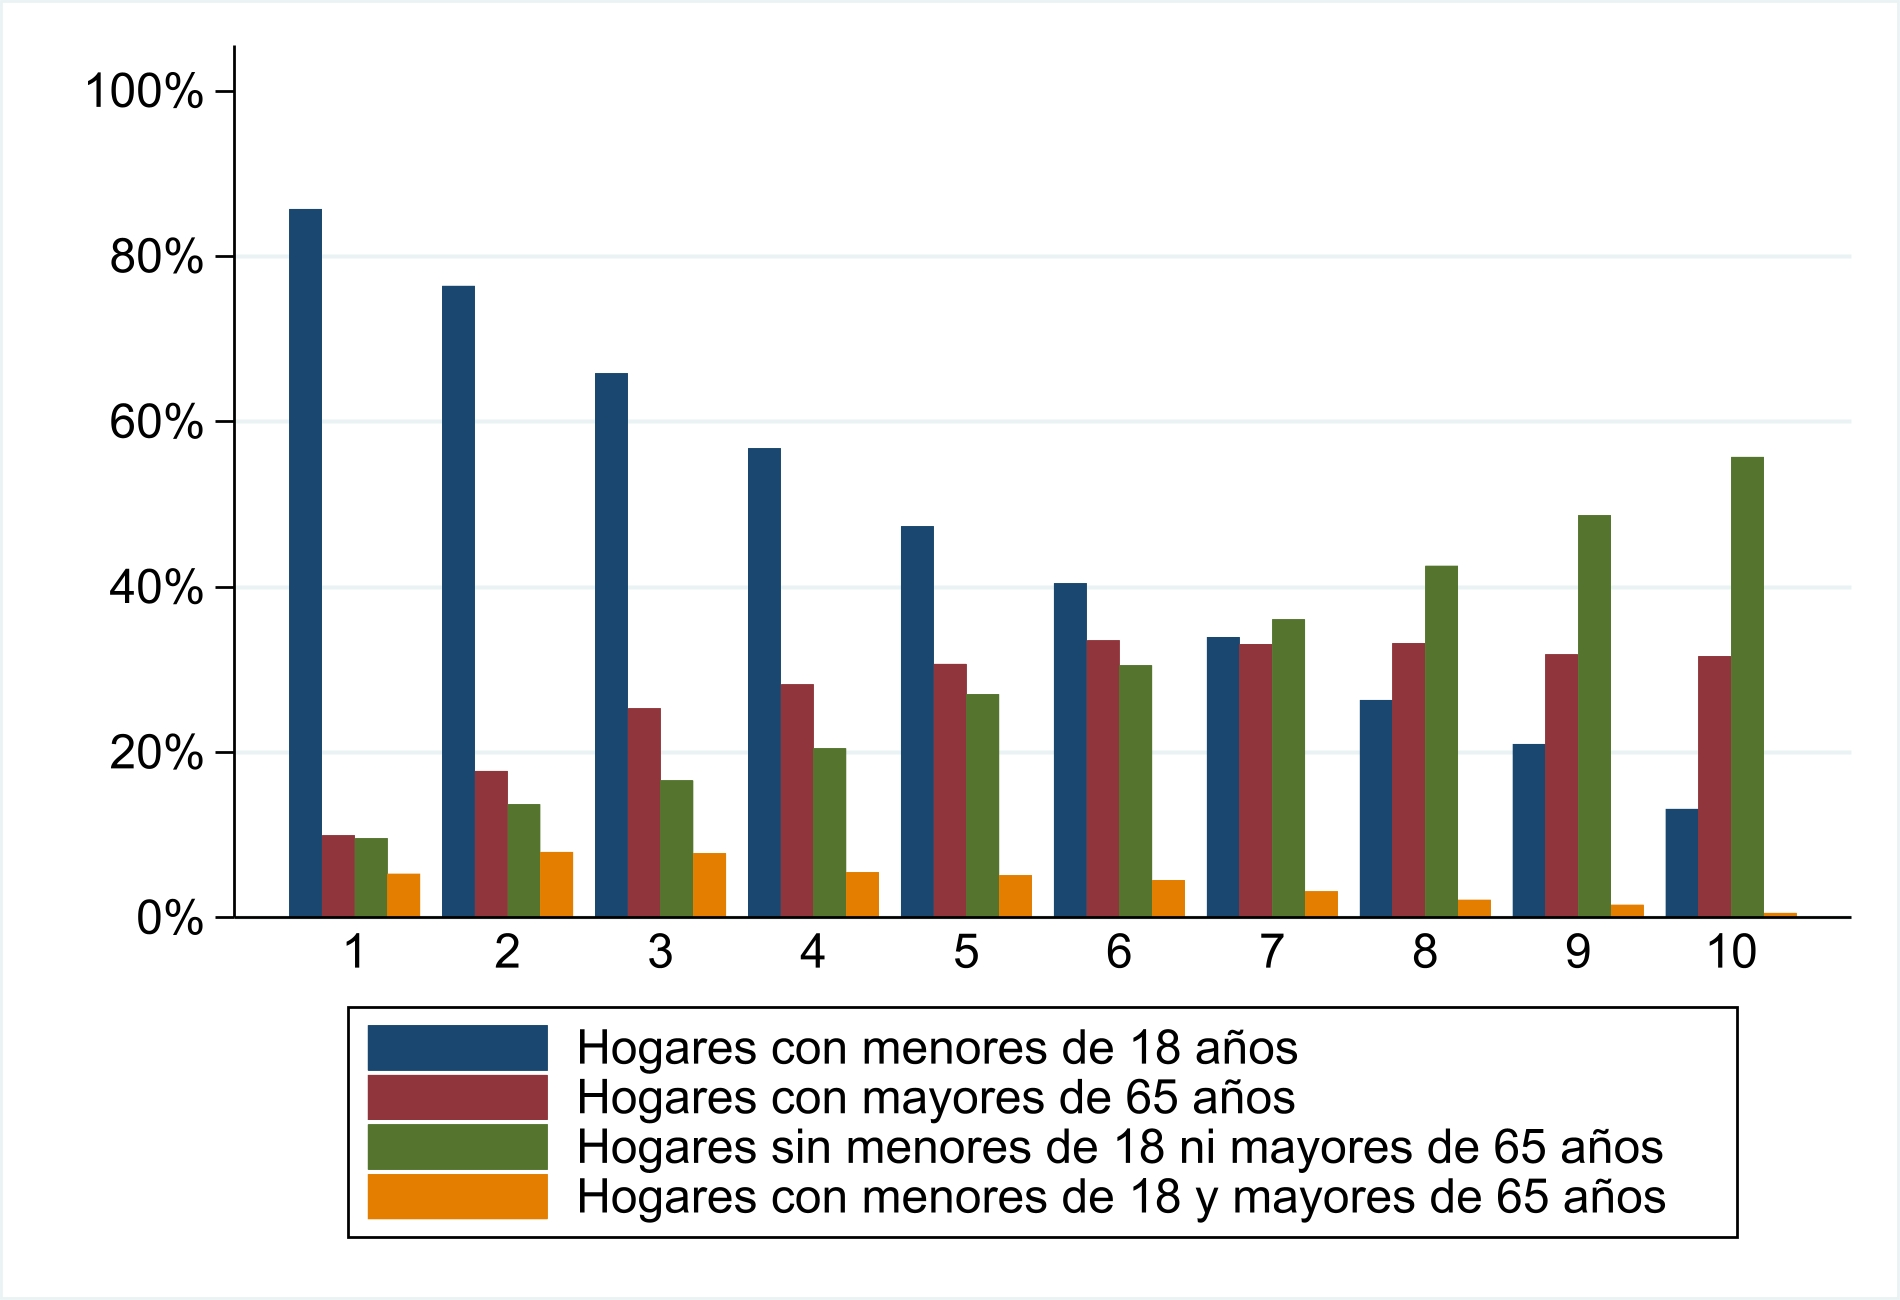
\includegraphics[scale=0.25]{imagenes/1 Composicion hogares 2011.jpg}
    \label{fig:imagen1}
\end{figure}
\vspace{3mm}

\subsection{Chequeos de robustez}

Lorem ipsum dolor sit amet, consectetur adipiscing elit, sed do eiusmod tempor incididunt ut labore et dolore magna aliqua. Ut enim ad minim veniam, quis nostrud exercitation ullamco laboris nisi ut aliquip ex ea commodo consequat. Duis aute irure dolor in reprehenderit in voluptate velit esse cillum dolore eu fugiat nulla pariatur. Excepteur sint occaecat cupidatat non proident, sunt in culpa qui officia deserunt mollit anim id est laborum.


\newpage

\section{Reflexiones finales / Conclusiones}

Lorem ipsum dolor sit amet, consectetur adipiscing elit, sed do eiusmod tempor incididunt ut labore et dolore magna aliqua. Ut enim ad minim veniam, quis nostrud exercitation ullamco laboris nisi ut aliquip ex ea commodo consequat. Duis aute irure dolor in reprehenderit in voluptate velit esse cillum dolore eu fugiat nulla pariatur. Excepteur sint occaecat cupidatat non proident, sunt in culpa qui officia deserunt mollit anim id est laborum.

Lorem ipsum dolor sit amet, consectetur adipiscing elit, sed do eiusmod tempor incididunt ut labore et dolore magna aliqua. Ut enim ad minim veniam, quis nostrud exercitation ullamco laboris nisi ut aliquip ex ea commodo consequat. Duis aute irure dolor in reprehenderit in voluptate velit esse cillum dolore eu fugiat nulla pariatur. Excepteur sint occaecat cupidatat non proident, sunt in culpa qui officia deserunt mollit anim id est laborum.

Lorem ipsum dolor sit amet, consectetur adipiscing elit, sed do eiusmod tempor incididunt ut labore et dolore magna aliqua. Ut enim ad minim veniam, quis nostrud exercitation ullamco laboris nisi ut aliquip ex ea commodo consequat. Duis aute irure dolor in reprehenderit in voluptate velit esse cillum dolore eu fugiat nulla pariatur. Excepteur sint occaecat cupidatat non proident, sunt in culpa qui officia deserunt mollit anim id est laborum.

\newpage


% Quinta parte:
% Bibliografía / Referencias. Estas líneas crean una sección de referencias y
% que aparezca dentro del índice
\cleardoublepage
\phantomsection
\addcontentsline{toc}{section}{Referencias}

% En este punto se especifica cuál es el archivo .bib que contiene toda la
% la bibliografía que se utiliza en la tesis
\bibliography{Bibliography}

% En caso de no querer usar el paquete natbib y el archivo .bib, se puede crear 
% la bibliografia a mano. En ese caso se podría hacer lo siguiente:

% \section{Referencias / Bibliografia} o \section*{Referencias / Bibliografia}

% Crear un nuevo archivo .tex en donde poner la bibliografía o incorporarla 
% abajo de aca. En caso de querer crear un archivo, podria ubicarse en la misma 
% direccion que main.tex entonces se pondria

% \input{bibliografia.tex}

\newpage


% Sexta parte: 
% Anexos. En caso de que no hayan anexos, se pueden comentar las lineas que
% vienen a continuación. Se pueden agregar más anexos si hacen faltas
\appendix
\section{Anexo}
\subsection{Mas informacion sobre los datos}

Lorem ipsum dolor sit amet, consectetur adipiscing elit, sed do eiusmod tempor incididunt ut labore et dolore magna aliqua. Ut enim ad minim veniam, quis nostrud exercitation ullamco laboris nisi ut aliquip ex ea commodo consequat. Duis aute irure dolor in reprehenderit in voluptate velit esse cillum dolore eu fugiat nulla pariatur. Excepteur sint occaecat cupidatat non proident, sunt in culpa qui officia deserunt mollit anim id est laborum.

Lorem ipsum dolor sit amet, consectetur adipiscing elit, sed do eiusmod tempor incididunt ut labore et dolore magna aliqua. Ut enim ad minim veniam, quis nostrud exercitation ullamco laboris nisi ut aliquip ex ea commodo consequat. Duis aute irure dolor in reprehenderit in voluptate velit esse cillum dolore eu fugiat nulla pariatur. Excepteur sint occaecat cupidatat non proident, sunt in culpa qui officia deserunt mollit anim id est laborum.

Lorem ipsum dolor sit amet, consectetur adipiscing elit, sed do eiusmod tempor incididunt ut labore et dolore magna aliqua. Ut enim ad minim veniam, quis nostrud exercitation ullamco laboris nisi ut aliquip ex ea commodo consequat. Duis aute irure dolor in reprehenderit in voluptate velit esse cillum dolore eu fugiat nulla pariatur. Excepteur sint occaecat cupidatat non proident, sunt in culpa qui officia deserunt mollit anim id est laborum.

\newpage

\subsection{Supuestos de la metodologia en detalle}

Lorem ipsum dolor sit amet, consectetur adipiscing elit, sed do eiusmod tempor incididunt ut labore et dolore magna aliqua. Ut enim ad minim veniam, quis nostrud exercitation ullamco laboris nisi ut aliquip ex ea commodo consequat. Duis aute irure dolor in reprehenderit in voluptate velit esse cillum dolore eu fugiat nulla pariatur. Excepteur sint occaecat cupidatat non proident, sunt in culpa qui officia deserunt mollit anim id est laborum.

Lorem ipsum dolor sit amet, consectetur adipiscing elit, sed do eiusmod tempor incididunt ut labore et dolore magna aliqua. Ut enim ad minim veniam, quis nostrud exercitation ullamco laboris nisi ut aliquip ex ea commodo consequat. Duis aute irure dolor in reprehenderit in voluptate velit esse cillum dolore eu fugiat nulla pariatur. Excepteur sint occaecat cupidatat non proident, sunt in culpa qui officia deserunt mollit anim id est laborum.

Lorem ipsum dolor sit amet, consectetur adipiscing elit, sed do eiusmod tempor incididunt ut labore et dolore magna aliqua. Ut enim ad minim veniam, quis nostrud exercitation ullamco laboris nisi ut aliquip ex ea commodo consequat. Duis aute irure dolor in reprehenderit in voluptate velit esse cillum dolore eu fugiat nulla pariatur. Excepteur sint occaecat cupidatat non proident, sunt in culpa qui officia deserunt mollit anim id est laborum.

\newpage

\end{document}
